%
% teil4.tex -- Beispiel-File für Teil 4
%
% (c) 2020 Prof Dr Andreas Müller, Hochschule Rapperswil
%
% !TEX root = ../../buch.tex
% !TEX encoding = UTF-8
%
\section{CWT und FFT im Vergleich
	\label{wavelets:section:teil4}}
\rhead{Teil 4}

In diesem Kapitel geht es darum sich mit den Möglichkeiten der CWT auseinander zu setzen. Im speziellen liegt das Interesse im Vergleich von der CWT zur FFT und wo sich Vor- und Nachteile der jeweiligen Transformation befinden. Dabei wird wieder mit kurz auftretenden Sinus-Sequenzen getestet.
Danach wird um das Ganze realistischer zu gestalten, dem Grundsignal noch ein weisses Rauschen beigemischt.

\subsection{Rauschfreies Signal
	\label{wavelets:subsection:CWTvsFFTRauschfrei}}
Es ist klar zu erkennen, wie FFT zeitlich den start und Endpunkt nicht exakt lokalisieren kann. Dem gegenüber ist die CWT in der Lage die Zeitpunkte eindeutig zu bestimmen. An der Stelle kommt die Phase als äusserst interessantes Werkzeug zum Zug. Die Wavelettransformation reagiert sehr sensible auf Änderungen im Signal und diese schlagartigen Wechsel lassen sich sehr deutlich identifizieren.
Damit die beiden Transformationen miteinander verglichen werden können müssen ihr grundsätzlichen Einstellungen gleich sein. Die FFT sowie CWT besitzen im vorliegenden Fall eine Auflösung von 1Hz und eine Überlappung von 50\% bezüglich der zeitlichen Verschiebung. Das ist insofern wichtig, weil beispielsweise eine FFT mit einer schlechteren Frequenzauflösung natürlich im Zeitbereich dementsprechend wieder besser performen würde.
Was dem gegenüber steht ist die Verschmierung der Frequenz durch die CWT. Die FFT schneidet bei der Genauigkeit der Frequenzbestimmung besser ab, d.h. bei der FFT besitzt im Rauschfreienfall nur die gesuchte Frequenz eine nennenswerte Amplitude. Dafür erhält man bei der CWT durch die Voraussetzung der endlichen Energie und die damit im Wavelet für jede Frequenz $k$ entsprechend korrekt verpackte Gewichtung, eine sehr präzise Reproduzierung der Amplitudenhöhe bei der Transformation in den Frequenzbereich. Die FFT schafft das nur wenn mit einem Rechteck-Fenster und genügend Periodizität des Signals. Mit Periodizität ist die Zeitdauer gemeint wie lange das Signal (Sinus bei Frequenz $k$Hz) konstant vorkommt. Bei der FFT ist das Fenster immer gleich breit, entsprechend der gewählten Auflösung (bei einem Herz muss die Periodizität des Signals also 1 Sekunde betragen damit der korrekte Amplitudenwert ausgegeben werden kann)(Abbildung \ref{wavelet:fig:FFTnoiseFree}).

\begin{figure}
	\centering
	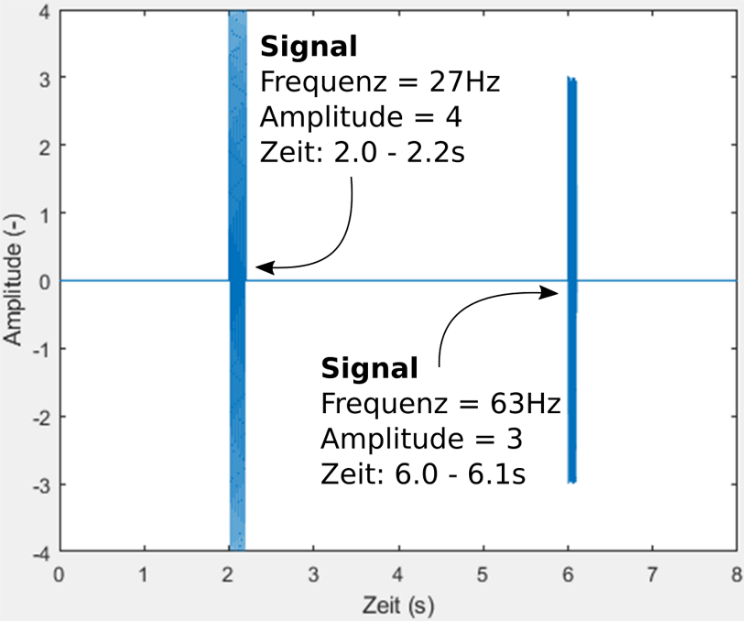
\includegraphics[width=0.3\textwidth]{papers/wavelets/images/18-1_CWTvsFFTSignal.png}
	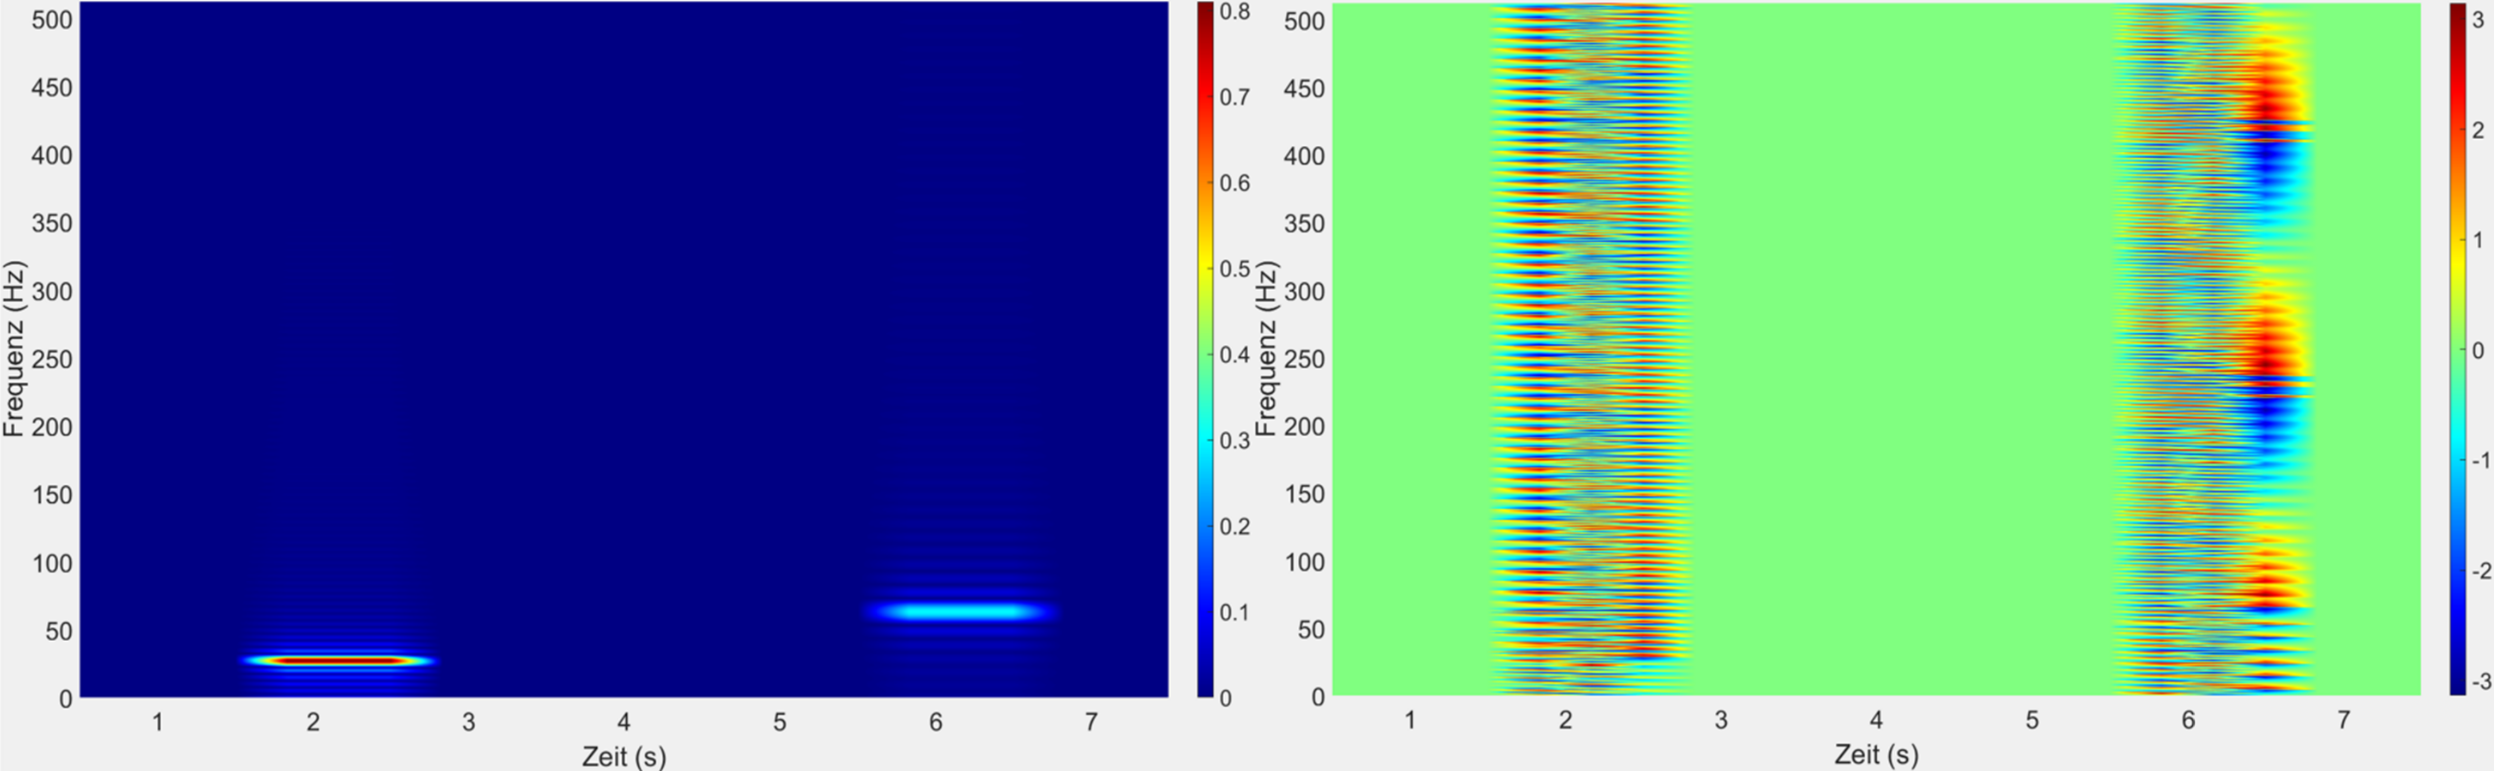
\includegraphics[width=\textwidth]{papers/wavelets/images/18-2_FFTnoiseFree.png}
	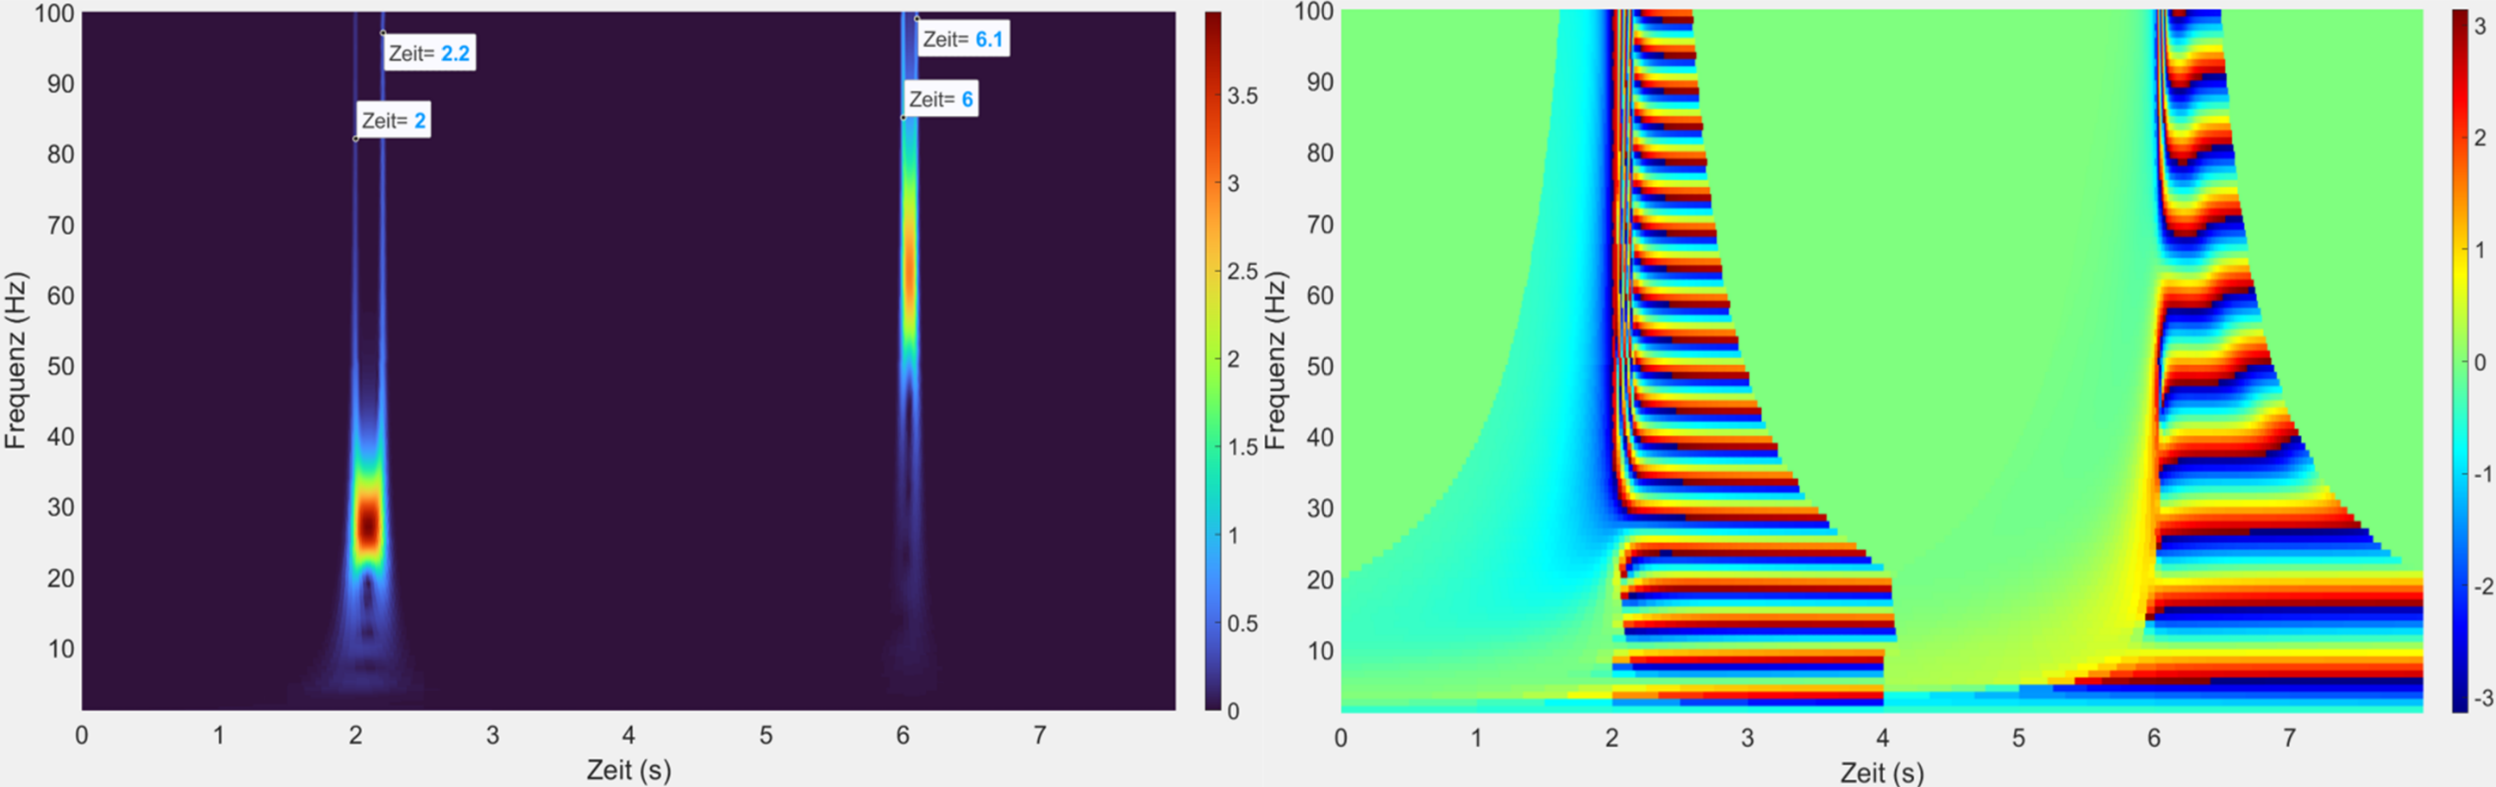
\includegraphics[width=\textwidth]{papers/wavelets/images/18-3_CWTnoiseFree.png}
	\caption{Amplituden- und Phasengang von FFT sowie CWT bei einem rauschfreien Signal.}
	\label{wavelet:fig:FFTnoiseFree}
\end{figure}

	
\subsection{Rauschbelastetes Signal
	\label{wavelets:subsection:CWTvsFFTRauschbelastet}}
Die FFT scheint durch das Rauschen weniger stark beeinflusst zu werden, die beiden Sinussignale werden in der Frequenz sauber detektiert, die Amplitude bleibt relativ unverändert, d.h. die Problematik mit der Kurzzeitigkeit der Signale verhindert ein genaues Reproduzieren der Amplituden der Zeitsignale und nicht das Rauschen.
Die CWT ist nach wie vor viel genauer in der zeitlichen Detektion, jedoch gehen zwei wichtige Eigenschaften im verrauschten Signal verloren:
\begin{itemize}
	\item Die Abbildung der scharfen Übergänge in den, dem Signal gegenüber höher liegenden Frequenzen im Amplitudengang.
	\item Die Möglichkeit zur zeitlichen Lokalisierung des Signales im Phasengang.
\end{itemize}
Das es zu diesem Ergebnis kommt, ist nicht wider erwarten, weil mit der Zufälligkeit des Rauschens zusätzliche abrupte Änderungen in und um die eigentlichen Signale gepackt werden. und solange das Signal sich nicht extrem deutlich durch seine Amplitude vom Rauschen abheben kann, diese Zufälligkeit starken Einfluss auf den Amplituden- sowie Phasengang nimmt.
Die Amplitudenhöhen der Signale werden aber nach wie vor hervorragend abgebildet. Die Verschmierung der Frequenz bleibt unverändert.
(Abbildung \ref{wavelet:fig:FFTnoisy})
	
\begin{figure}
	\centering
	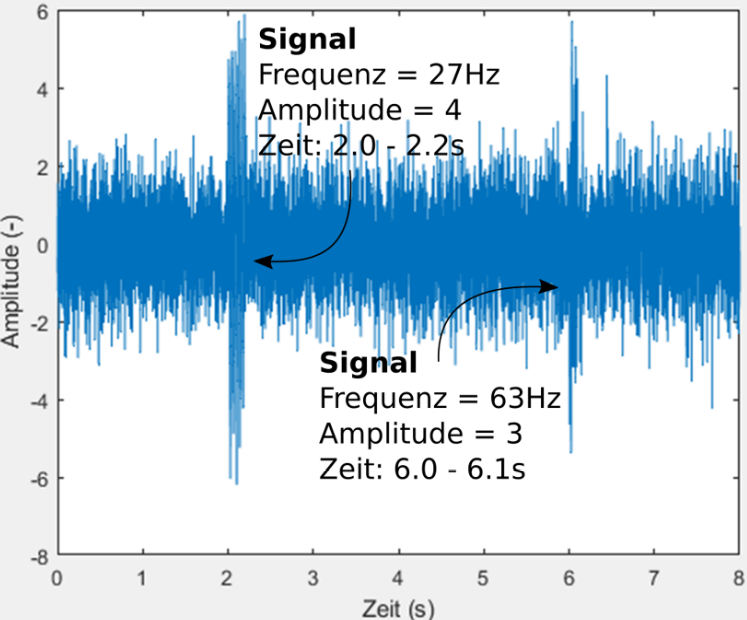
\includegraphics[width=0.3\textwidth]{papers/wavelets/images/18-4_CWTvsFFTSignalNoisy.png}
	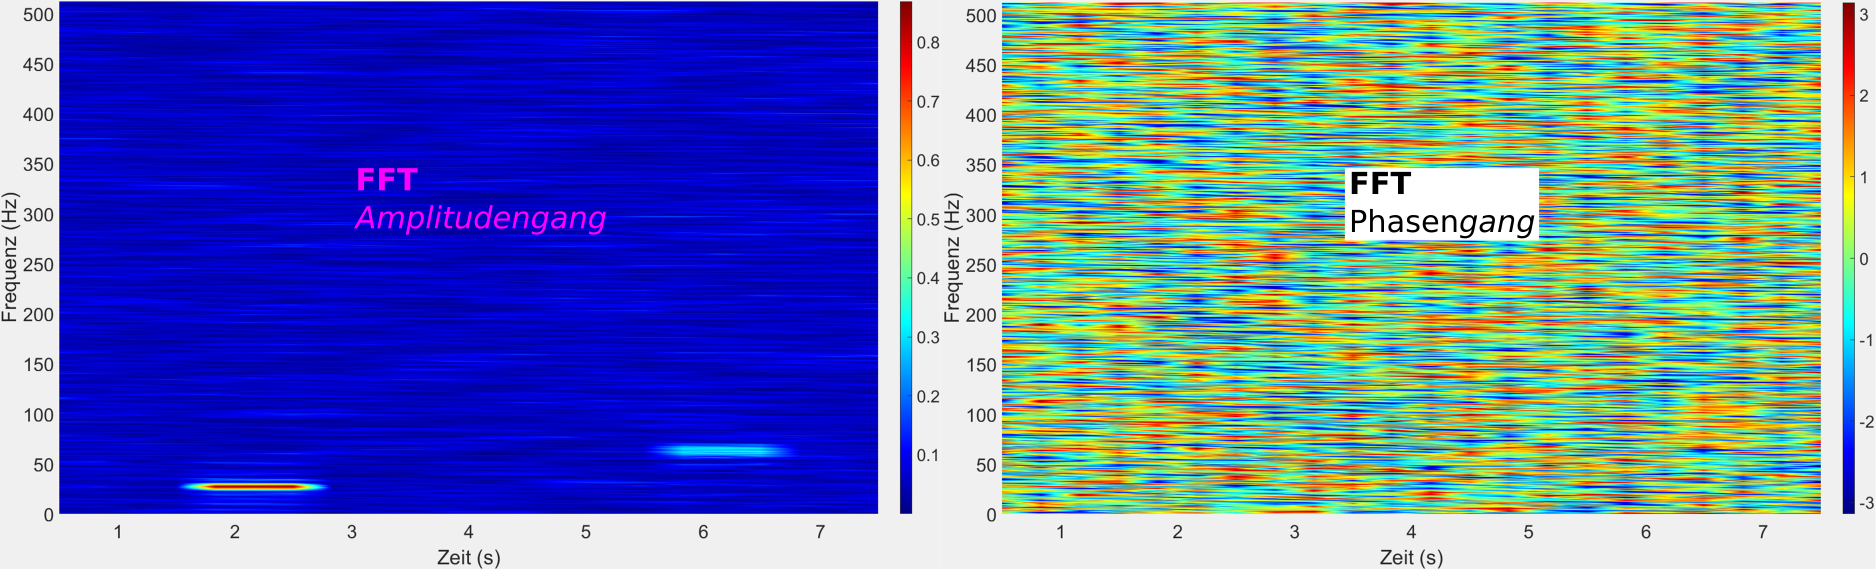
\includegraphics[width=\textwidth]{papers/wavelets/images/18-5_FFTnoisy.png}
	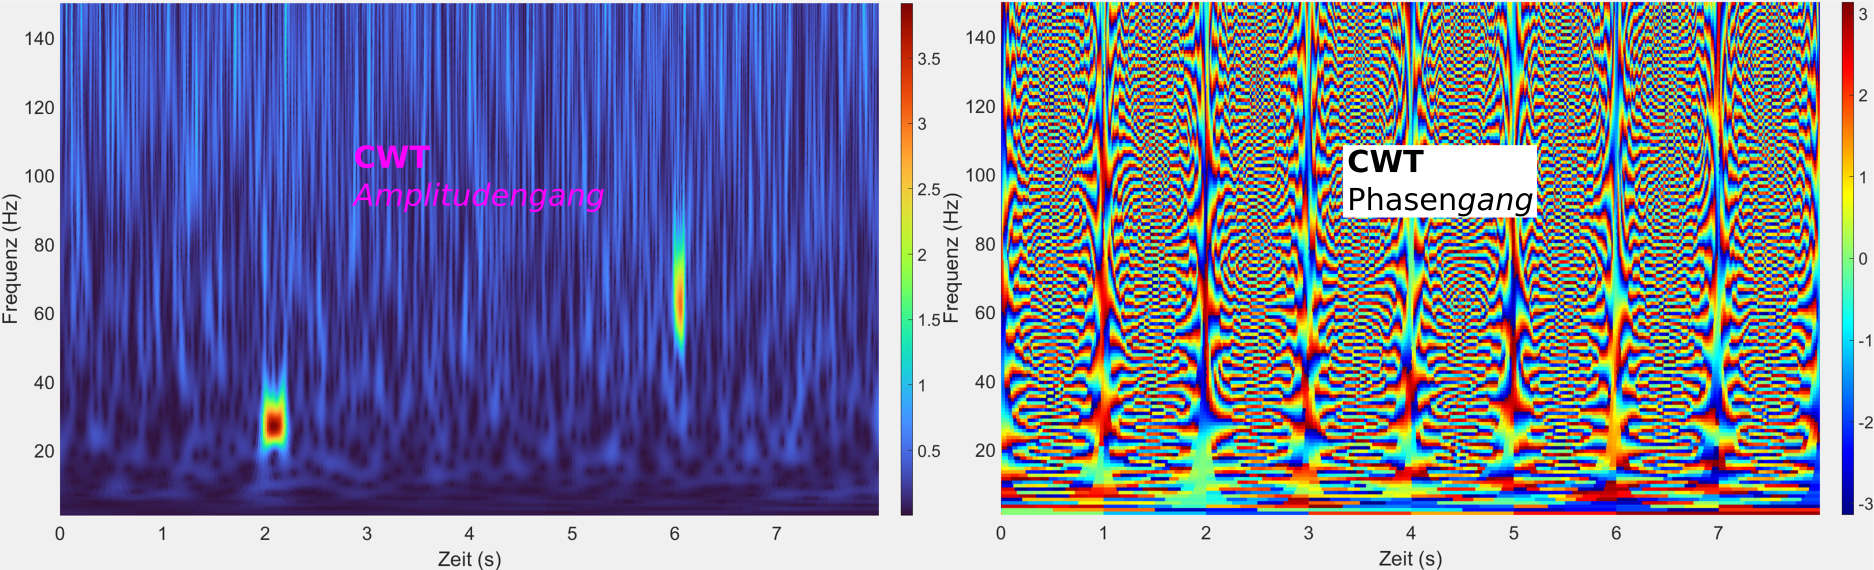
\includegraphics[width=\textwidth]{papers/wavelets/images/18-6_CWTnoisy.png}
	\caption{Amplituden- und Phasengang von FFT sowie CWT bei einem rauschbelasteten (weisses Rauschen) Signal.}
	\label{wavelet:fig:FFTnoisy}
\end{figure}
